\documentclass[]{article}
\usepackage[spanish.mexico]{babel}
\usepackage[T1]{fontenc}
\usepackage[utf8]{inputenc}
%\usepackage{lmodern}
\usepackage[a4paper]{geometry}

%Graficos e imagenes
\usepackage{graphicx}
%\graphicspath{ Imagenes/ }

\usepackage{cite}

%Grafico de barras
%\usepackage{pgfplots}


\usepackage{tikz}
\usepackage[american voltages, american currents,siunitx]{circuitikz}

%\title{Proyecto de Optimización de Energía}
%\author{Pablo Vivar Colina}
%\date{Mayo 2018}



\begin{document}
	
%\usepackage[top=2cm,bottom=2cm,left=1cm,right=1cm]{geometry}


\begin{titlepage}
     \begin{center}
	
\includegraphics[width=0.09\textwidth]{UNAM}\Large Universidad Nacional Autónoma de México
        	
\includegraphics[width=0.09\textwidth]{FI}\\[1cm]
        \Large Facultad de Ingeniería\\[1cm]
       % \Large División de Ciencias Básicas\\[1cm]
         \Large Laboratorio de Fundamentos de Control(6655)\\[1cm]
         %la clave antes era:4314
         \footnotesize Profesor: Salcedo Ubilla María Leonor Ing.\\[1cm]
        \footnotesize Semestre 2019-1\\[1cm]
        
       

        \Large Práctica No. 1\\[1cm]
        
           

\Large Introdcción MATLAB
        
         %Texto a la derecha
          \begin{flushright}
\footnotesize  Grupo 2\\[0.5cm]
\footnotesize Brigada: 4\\[0.5cm]
\footnotesize Rodrigo Adrián Martínez López\\[0.5cm]
\footnotesize Vivar Colina Pablo\\[0.5cm]
 \end{flushright}
    %Texto a la izquierda
          \begin{flushleft}
        \footnotesize Ciudad Universitaria Agosto de 2018.\\
          \end{flushleft}
         
          
        %\vfill
        %\today
   \end{center}
\end{titlepage}
 %agregar portada

%\maketitle

\tableofcontents  % Write out the Table of Contents

%\listoffigures  % Write out the List of Figures

\section{Resumen}

\section{Introducción}


\subsection{NI ELVIS}

Para crear una aplicación completa de NI ELVIS, explore otras soluciones de laboratorio para NI ELVIS.\\

Proporciona una experiencia de aprendizaje basada en proyectos, usando medidas en línea y diseño práctico y embebido.\\

El NI Educational Laboratory Virtual Instrumentation Suite (NI ELVIS) es un dispositivo modular de laboratorio educativo de ingeniería desarrollado específicamente para la academia. Con este enfoque práctico, los profesores pueden ayudar a los estudiantes a aprender habilidades de ingeniería prácticas y experimentales. NI ELVIS incluye un osciloscopio, multímetro digital, generador de funciones, fuente de alimentación variable, analizador de Bode y otros instrumentos comunes de laboratorio. Puede conectar una PC al NI ELVIS usando USB y desarrollar circuitos en su protoboard desmontable.\cite{NationalInstruments2018}\\


\section{Objetivos}

	\begin{itemize}
			\item Utilizar la herramientas de National Instruments para verificar las ecuaciones de función de transferencia
	\end{itemize}


\section{Materiales y métodos}

	\begin{itemize}
		\item NI Elvis
		\item Computadora con Suite de herramientas Texas Instruments
	\end{itemize}
	
\section{Resultados}


\begin{figure}[h!]
	\centering
	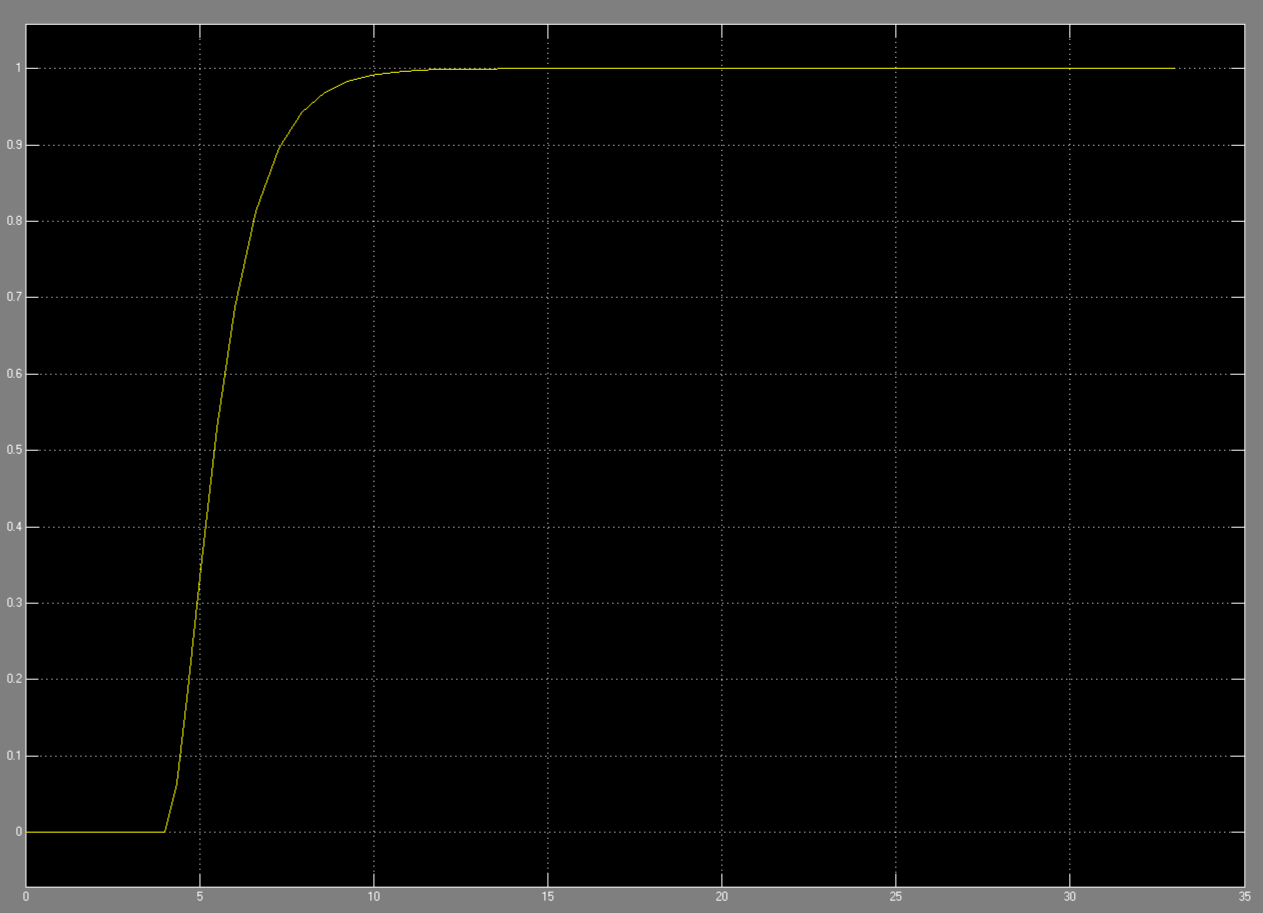
\includegraphics[width=0.6\textwidth]{Imagenes/FuncionTransferenciaCeroTreintaEscalon}
	\caption{FuncionTransferenciaCeroTreintaEscalon}
	\label{fig:FuncionTransferenciaCeroTreintaEscalon}
\end{figure}

\begin{figure}[h!]
	\centering
	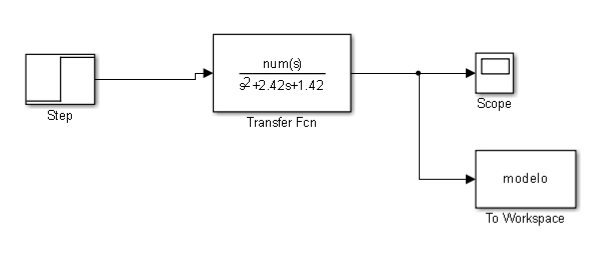
\includegraphics[width=0.6\textwidth]{Imagenes/FuncionTransferenciaCeroTreintaEscalonModelo}
	\caption{FuncionTransferenciaCeroTreintaEscalonModelo}
	\label{fig:FuncionTransferenciaCeroTreintaEscalonModelo}
\end{figure}

\begin{figure}[h!]
	\centering
	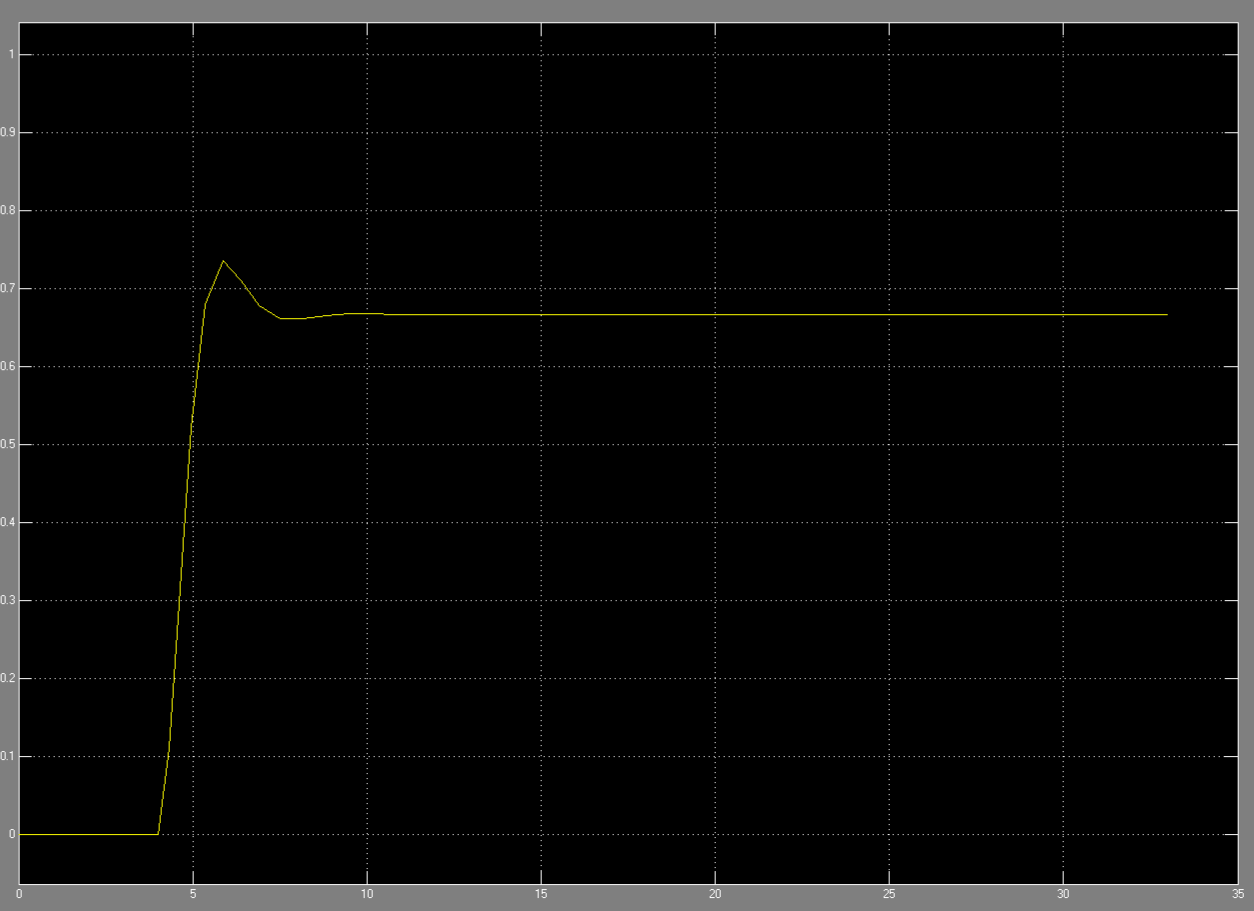
\includegraphics[width=0.6\textwidth]{Imagenes/FuncionTransferenciaCeroTreintaEscalonSumagain2Graf}
	\caption{FuncionTransferenciaCeroTreintaEscalonSumagain2Graf}
	\label{fig:FuncionTransferenciaCeroTreintaEscalonSumagain2Graf}
\end{figure}

\begin{figure}[h!]
	\centering
	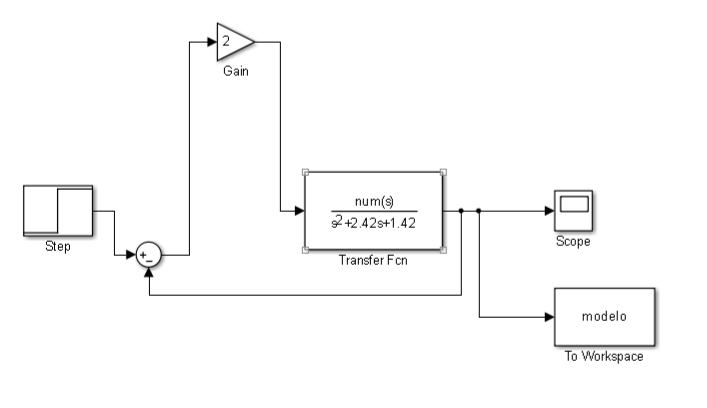
\includegraphics[width=0.6\textwidth]{Imagenes/FuncionTransferenciaCeroTreintaEscalonSumagain2modelo}
	\caption{FuncionTransferenciaCeroTreintaEscalonSumagain2modelo}
	\label{fig:FuncionTransferenciaCeroTreintaEscalonSumagain2modelo}
\end{figure}

\begin{figure}[h!]
	\centering
	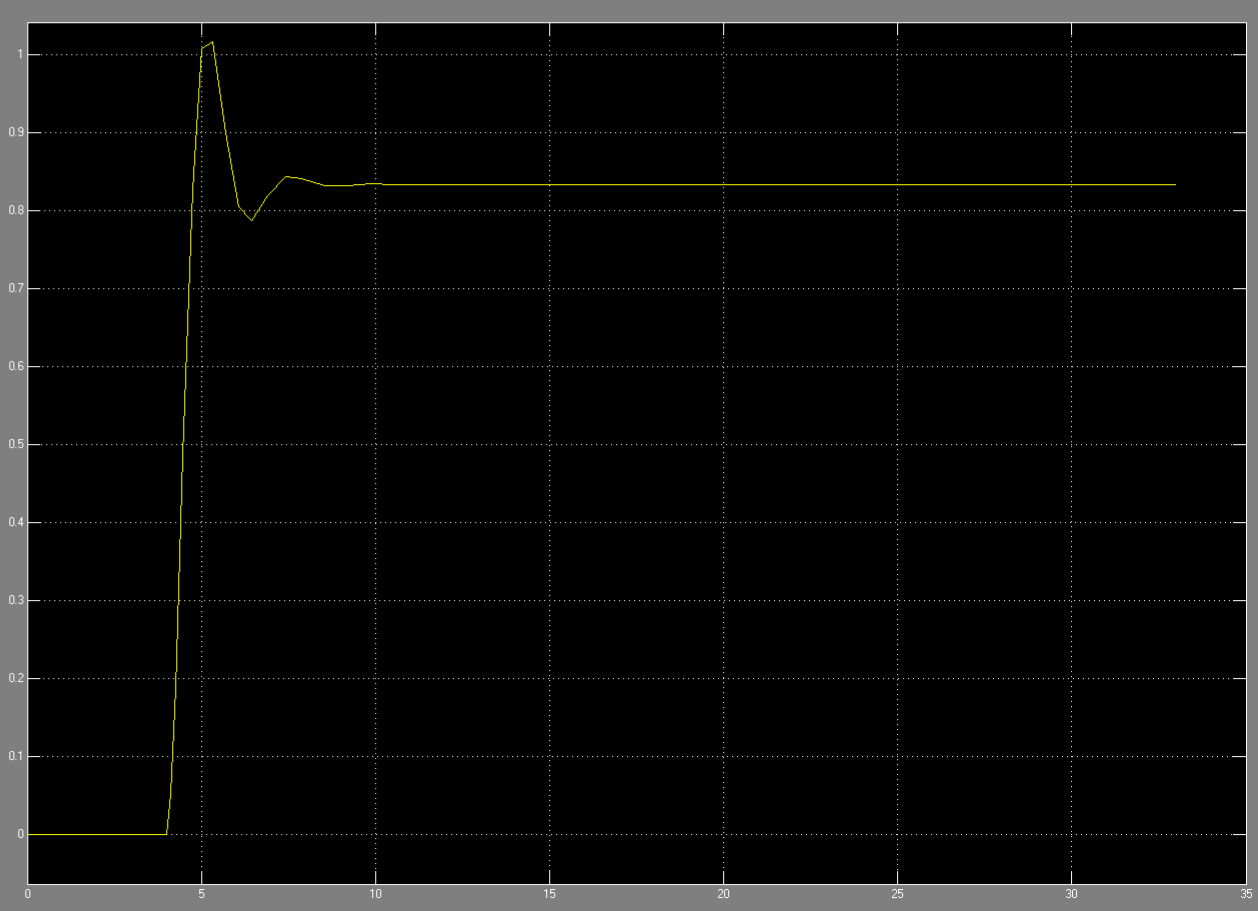
\includegraphics[width=0.6\textwidth]{Imagenes/FuncionTransferenciaCeroTreintaEscalonSumagain5Graf}
	\caption{FuncionTransferenciaCeroTreintaEscalonSumagain5Graf}
	\label{fig:FuncionTransferenciaCeroTreintaEscalonSumagain5Graf}
\end{figure}
FuncionTransferenciaCeroTreintaEscalonSumagain5modelo

\begin{figure}[h!]
	\centering
	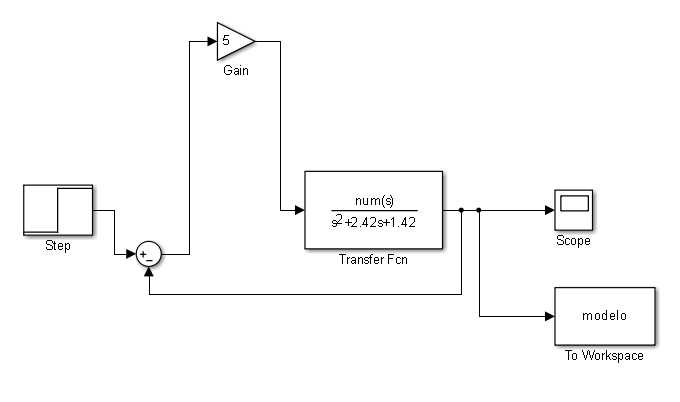
\includegraphics[width=0.6\textwidth]{Imagenes/FuncionTransferenciaCeroTreintaEscalonSumagain5modelo}
	\caption{FuncionTransferenciaCeroTreintaEscalonSumagain5modelo}
	\label{fig:FuncionTransferenciaCeroTreintaEscalonSumagain5modelo}
\end{figure}

\begin{figure}[h!]
	\centering
	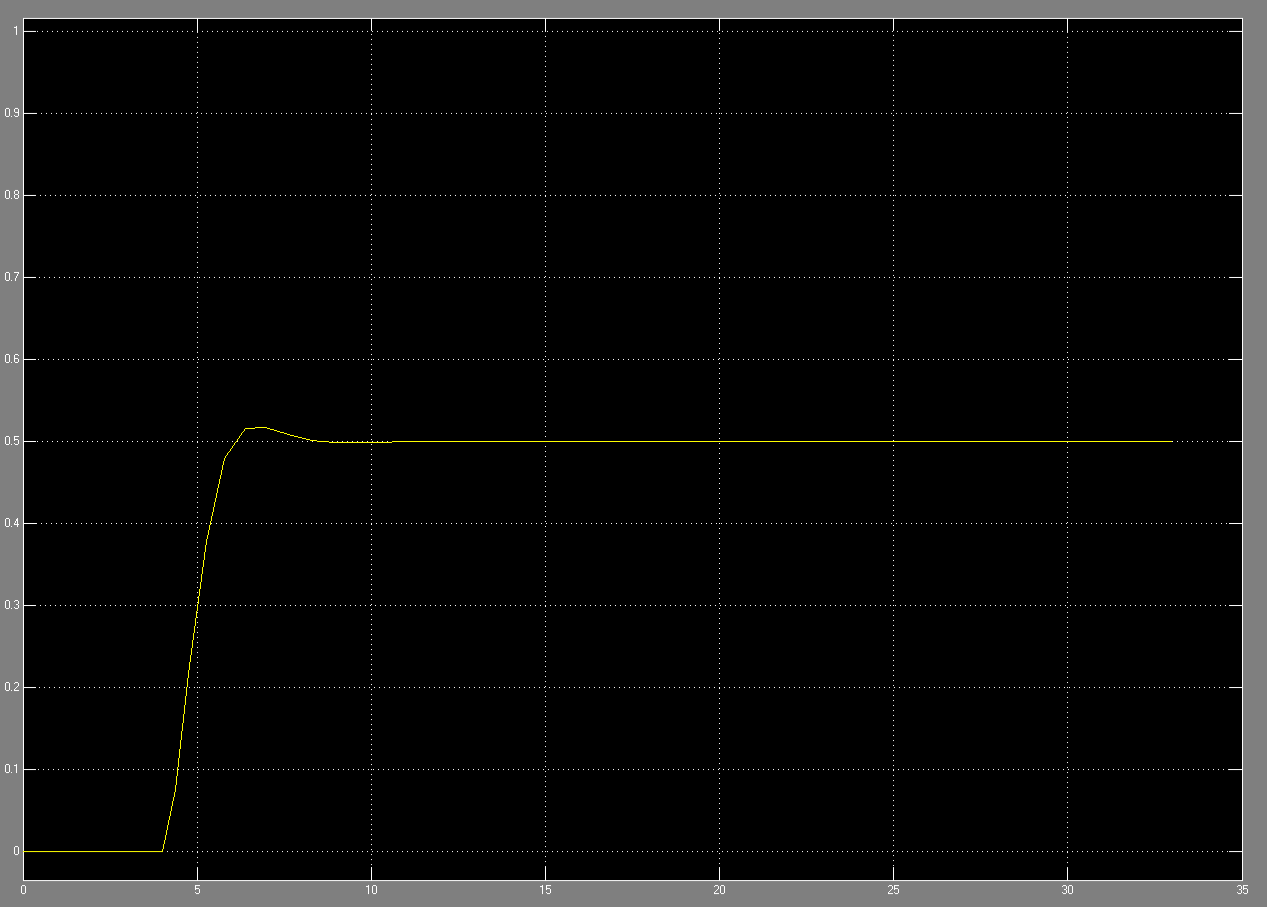
\includegraphics[width=0.6\textwidth]{Imagenes/FuncionTransferenciaCeroTreintaEscalonSumaGraf}
	\caption{FuncionTransferenciaCeroTreintaEscalonSumaGraf}
	\label{fig:FuncionTransferenciaCeroTreintaEscalonSumaGraf}
\end{figure}

\begin{figure}[h!]
	\centering
	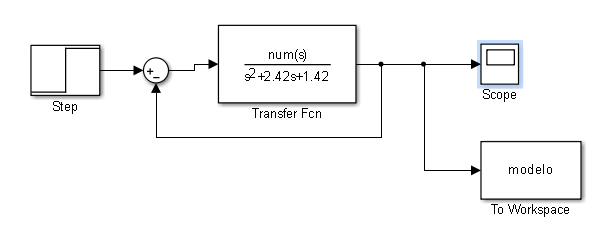
\includegraphics[width=0.6\textwidth]{Imagenes/FuncionTransferenciaCeroTreintaEscalonSumaModelo}
	\caption{FuncionTransferenciaCeroTreintaEscalonSumaModelo}
	\label{fig:FuncionTransferenciaCeroTreintaEscalonSumaModelo}
\end{figure}

\begin{figure}[h!]
	\centering
	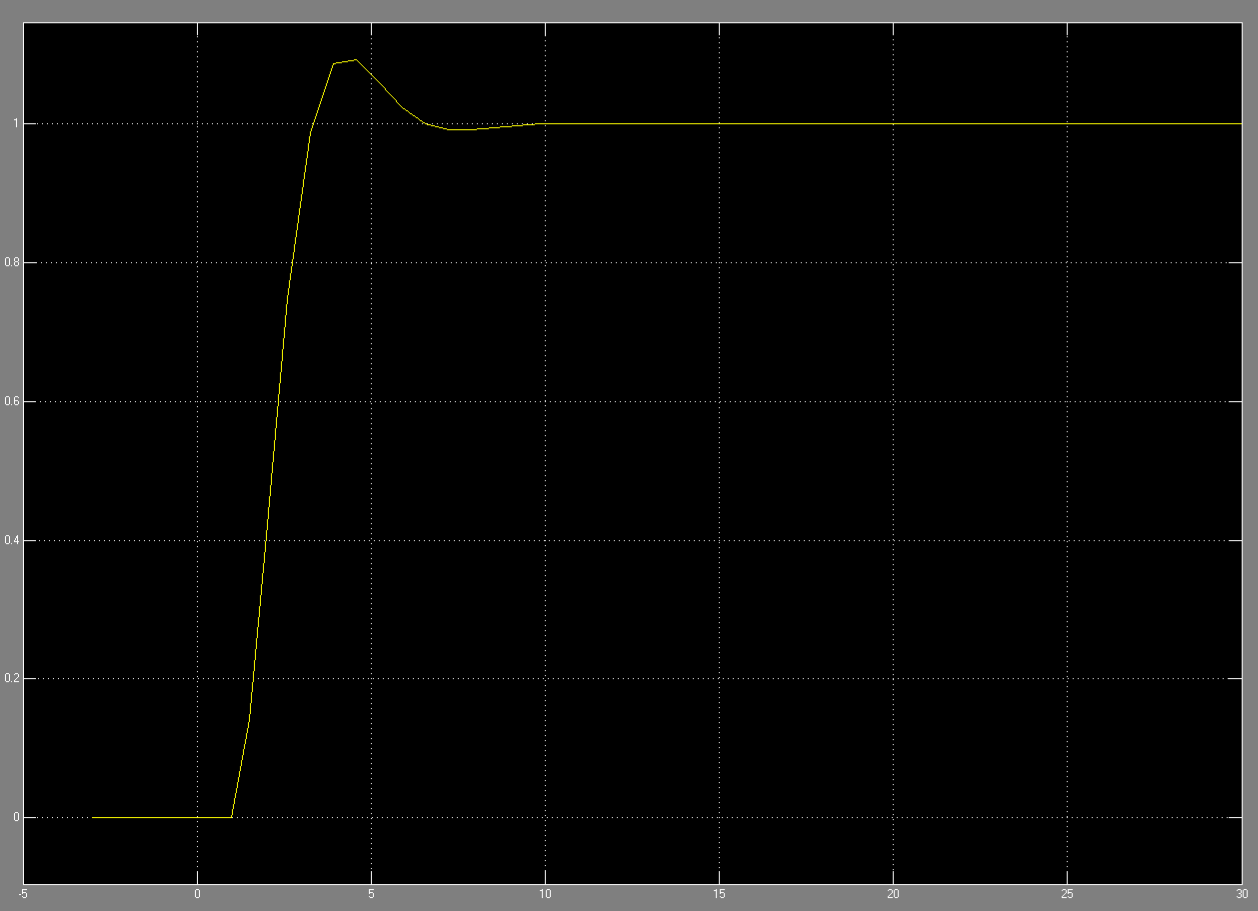
\includegraphics[width=0.6\textwidth]{Imagenes/FuncionTransferenciaCeroTreintaEscalonSumaPIDGraf}
	\caption{FuncionTransferenciaCeroTreintaEscalonSumaPIDGraf}
	\label{fig:FuncionTransferenciaCeroTreintaEscalonSumaPIDGraf}
\end{figure}

\begin{figure}[h!]
	\centering
	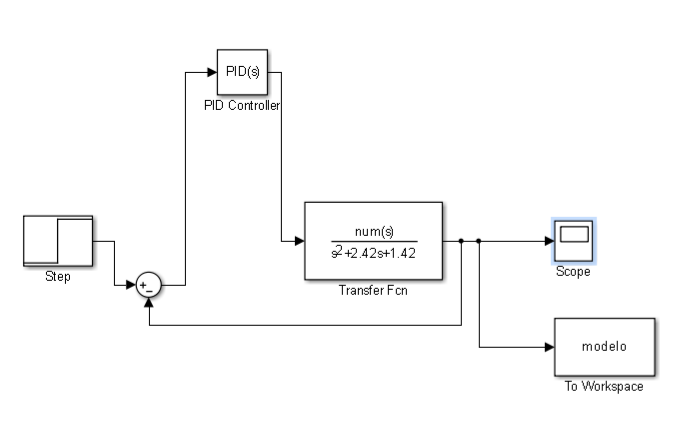
\includegraphics[width=0.6\textwidth]{Imagenes/FuncionTransferenciaCeroTreintaEscalonSumaPIDmodelo}
	\caption{FuncionTransferenciaCeroTreintaEscalonSumaPIDmodelo}
	\label{fig:FuncionTransferenciaCeroTreintaEscalonSumaPIDmodelo}
\end{figure}



\begin{figure}[h!]
	\centering
	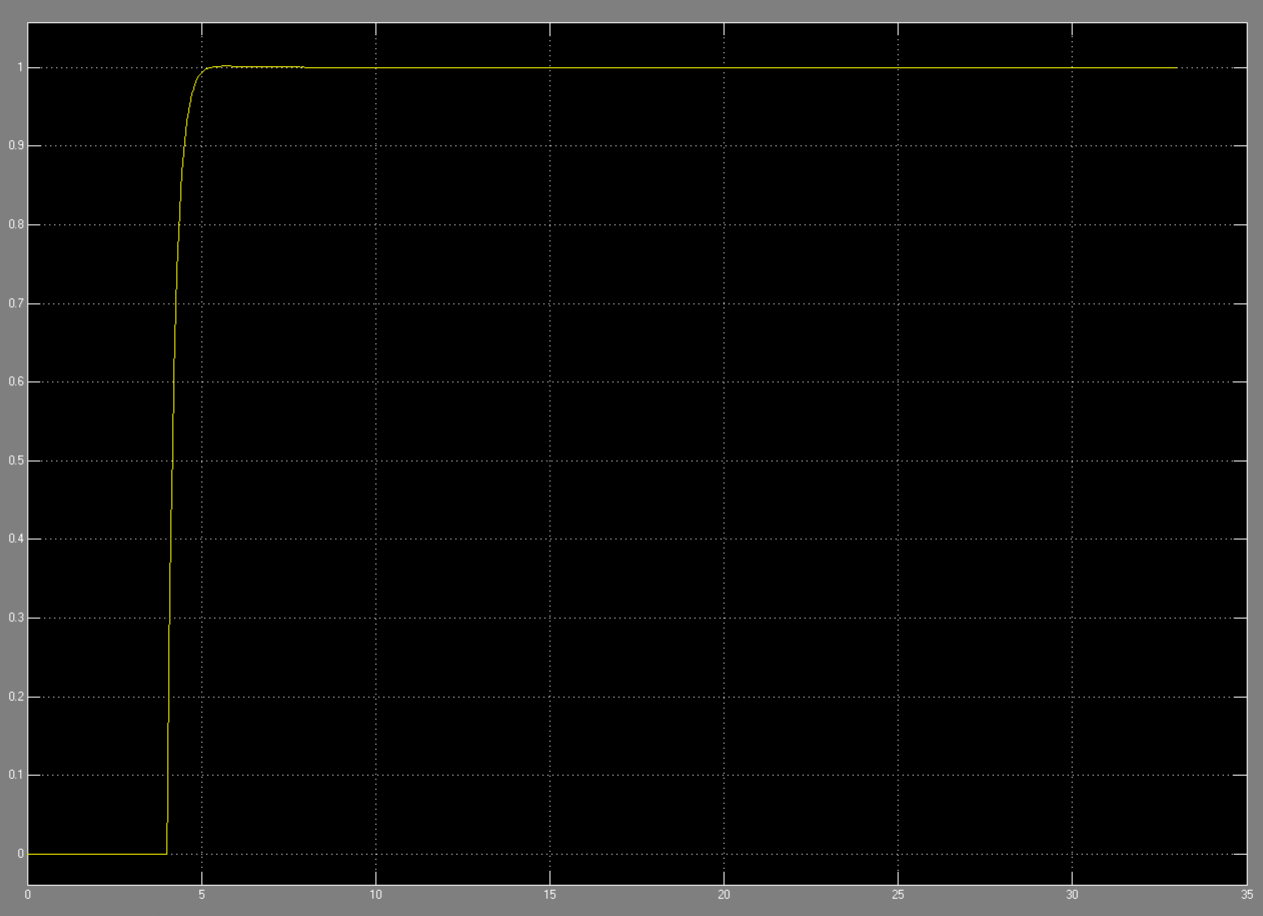
\includegraphics[width=0.6\textwidth]{Imagenes/FuncionTransferenciaPIDgrafP7p5I4p5D3p0}
	\caption{FuncionTransferenciaPIDgrafP7p5I4p5D3p0}
	\label{fig:FuncionTransferenciaPIDgrafP7p5I4p5D3p0}
\end{figure}

\begin{figure}[h!]
	\centering
	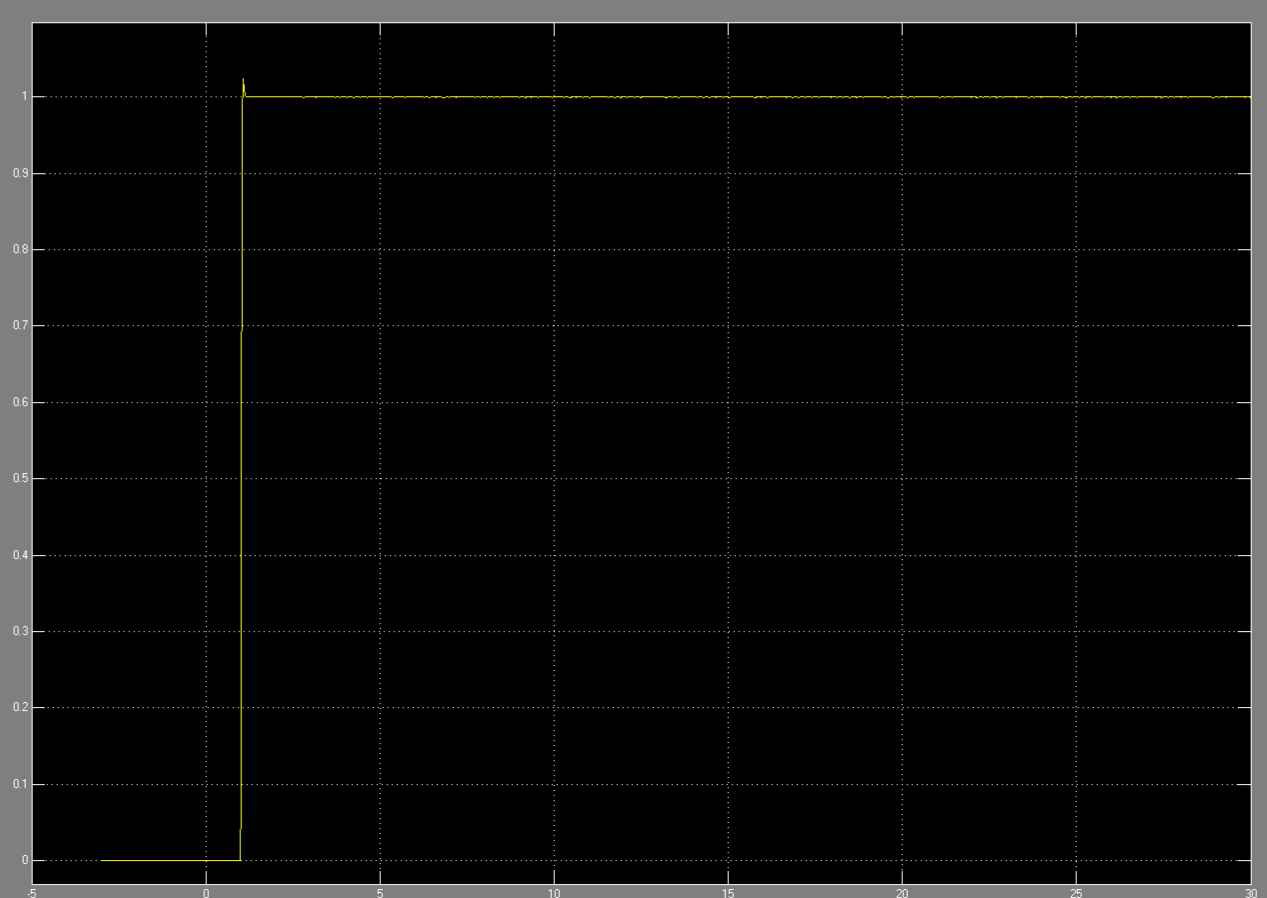
\includegraphics[width=0.6\textwidth]{Imagenes/FuncionTransferenciaPIDgrafP75I45D30}
	\caption{FuncionTransferenciaPIDgrafP75I45D30}
	\label{FuncionTransferenciaPIDgrafP75I45D30}
\end{figure}



\begin{equation}
A(dB)=20log_{10}\frac{V_s}{V_e}
\end{equation}




\begin{table}[h!]
	\centering
	\begin{tabular}{|c|c|c|c|}
		\hline
		Frecuencia [Hz] & $V_s$    & $V_e$    & A [db]    \\ \hline
		10                  & 3.737   & 0.3877  & 19.6805459368 \\ \hline
		100                 & 3.774   & 0.39111 & 19.6900595117 \\ \hline
		1000                & 3.132   & 0.387   & 18.1622157673 \\ \hline
		5000                & 1.174   & 0.39531 & 9.4546059251  \\ \hline
		10000               & 0.6331  & 0.3827  & 4.3722770259  \\ \hline
		15000               & 0.41214 & 0.37859 & 0.737512567   \\ \hline
		20000               & 0.31739 & 0.3911  & -1.8138915325 \\ \hline
		30000               & 0.21671 & 0.3827  & -4.9395902018 \\ \hline
		100000              & 0.6787  & 0.37405 & 5.1749638022  \\ \hline
	\end{tabular}
	\label{ATabla}
\end{table}






\section{Análisis de Resultados}



\section{Conclusiones}


\section{Referencias}

\bibliographystyle{plain}
\bibliography{Referencias.bib}



\end{document}
